% Auswertung Emissionssektrum:
% Grenzwinkel: 5,6°
% min. Wellenänge: 39,31 pm
% max. Energie Bremsberg: 31,54 keV
% Auswertung Detailspektrum
% K_beta Linie Halbwertsbreite: 0,4°
% K_beta Linie min: 20,10° mit Energie 8956,705134376347eV
% K_beta Linie max: 20,50° mit Energie 8789,245217800455eV
% K_beta Linie max: 20,20° mit Energie 8914,203896517447eV
% K_beta Auflösungsvermögen A: 53,23186634025094
% ----------------
% K_alpha Linie Halbwertsbreite: 0,45°
% K_alpha Linie min: 22,30° mit Energie 8111,763305657744eV
% K_alpha Linie max: 22,75° mit Energie 7959,584434702297eV
% K_alpha Linie max: 22,60° mit Energie 8009,617524536037eV
% K_alpha Auflösungsvermögen A: 52,63291463688781
% ----------------
% sigma_1 exp: 3,5713015465602105
% sigma_2 exp: 12,22058064763327
% sigma_3 exp: 22,0875728042239
% ----------------
% sigma_1 theo: 3,5713015465602105
% sigma_2 theo: 12,138311271922081
% sigma_3 theo: 24,039726162119393
% ----------------
% Theta_K_Sr_exp: 10,99°
% Theta_K_Zr_exp: 9,91°
% Theta_K_Br_exp: 13,13°
% Theta_K_Zn_exp: 19,84°
% Theta_K_Ga_exp: 17,21°
% ----------------
% E_Sr exp: 16146,119558680297 eV
% E_Zr exp: 17885,183610259875 eV
% E_Br exp: 13550,104011791671 eV
% E_Zn exp: 9069,259432194094 eV
% E_Ga exp: 10403,247695213902 eV
% ----------------
% sigma_Sr exp: 4,326405561581936
% sigma_Zr exp: 4,606220593256381
% sigma_Br exp: 4,098435453201631
% sigma_Zn exp: 4,6679672621877195
% sigma_Ga exp: 3,8674501840169953
% ----------------
% a_sqrt: 3,828+/-0,009
% Rydberg exp(a): 14,65+/-0,07 eV
% b_sqrt: -1,81+/-0,28
% b: 3,3+/-1,0
\section{Auswertung}
\label{sec:Auswertung}
\subsection{Überprüfung der Bragg Bedingung}
In Abbildung (\ref{fig:Bragg}) sind die Messdaten zur Überprüfung der
Bragg-Bedingung der Röntgenstahlen auf ein LiF-Gitter dargestellt.
Anhand dieser Abbildung wird das Maximum bei $\theta_{\text{exp.}} = 14\,\unit{\degree}$
abgelesen. Der theoretische Braggwinkel lautet $\theta_{\text{theo.}} = 14\,\unit{\degree}$.
\begin{figure}[H]
  \centering
  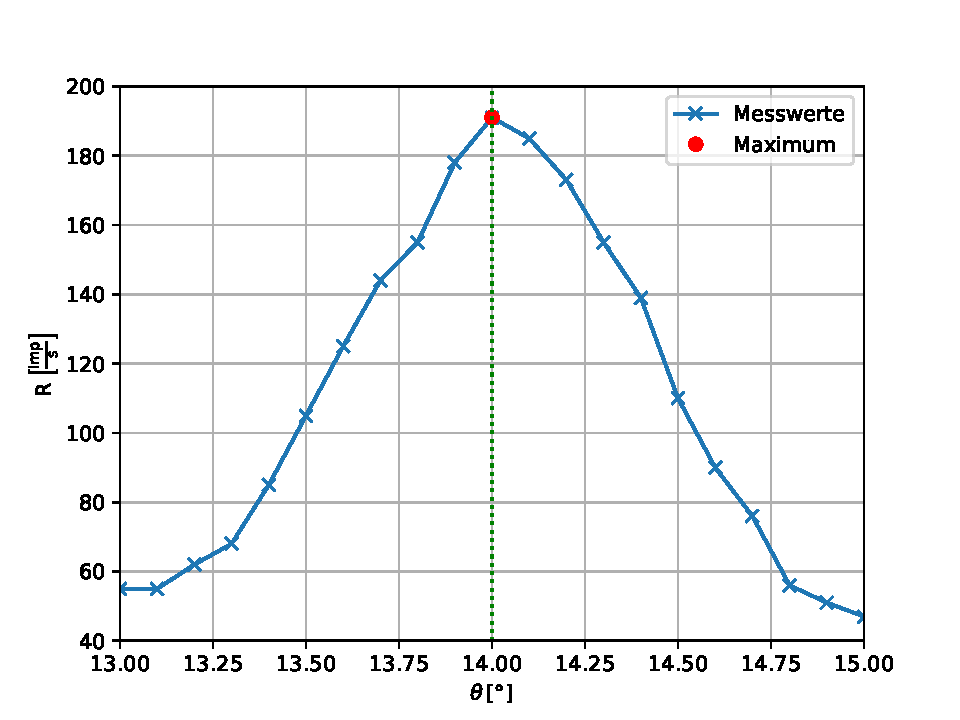
\includegraphics{content/Plots/Bragg.pdf}
  \caption{Messdaten zur Überprüfung der Bragg-Bedinung.}
  \label{fig:Bragg}
\end{figure}

\subsection{Emissionsspektrum einer Cu-Röntgenröhre}
Die Messdaten des Emissionsspektrums einer Cu-Röntgenröhre sind in der 
Abbildung (\ref{fig:Emissionsspektrum}) abgebildet. Zusätzlich sind in dieser
Abbildung der Bremsberg, die $K_{\alpha}$- und $K_{\beta}$-Linien markiert.
Aus der Graphik lassen sich 
\begin{align*}
  K_{\alpha} &= 22,6\,\unit{\degree} \\
  K_{\alpha} &= 20,2\,\unit{\degree}
\end{align*}
bestimmen. Der abgelesene Grenzwinkel $\theta_{\text{Grenz}}$ lautet etwa
$$\theta_{\text{Grenz}} = 5,6\,\unit{\degree}\,.$$ Damit lässt sich durch Umstellen der Gleichung
(\ref{eqn:Bragg_Bedingung}) die minimale Wellenlänge und mit der Gleichungen (\ref{eqn:lambda}) und (\ref{eqn:E_kin}) die maximale Energie des Bremsbergs
berechnen. Daraus folgt
\begin{align*}
  \lambda_{\text{min}} &= 39,31\,\unit{\pico\metre}\\
  E_{\text{max}} &= 31,54\,\unit{\kilo\eV}\,.
\end{align*}

\begin{figure}[H]
  \centering
  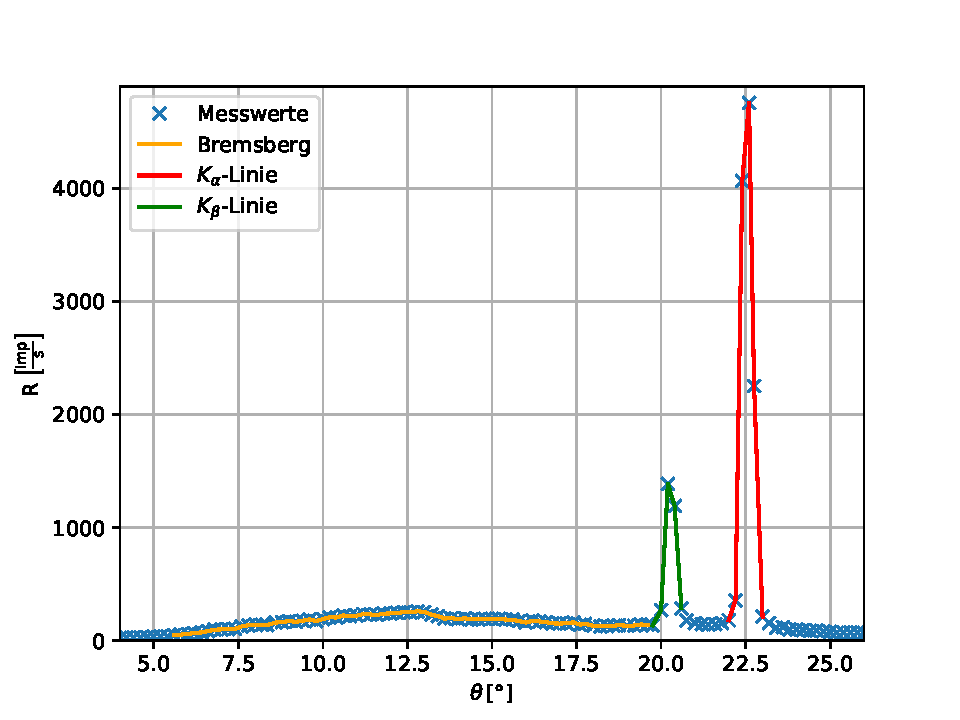
\includegraphics{content/Plots/Emissionsspektrum.pdf}
  \caption{Messdaten des Emissionsspektrum einer Cu-Röhre.}
  \label{fig:Emissionsspektrum}
\end{figure}
Um das Auflösungsvermögen der Apparatur zu bestimmen, wird der Ausschnitt der $K_{\alpha}$-
und $K_{\beta}$-Linien in der Abbildung (\ref{fig:Detailspektrum}) dargestellt. Innerhalb dieser Abbildung
sind die Halbwertsbreiten der $K_{\alpha}$ und $K_{\beta}$-Linien eingezeichnet. 
\begin{figure}[H]
  \centering
  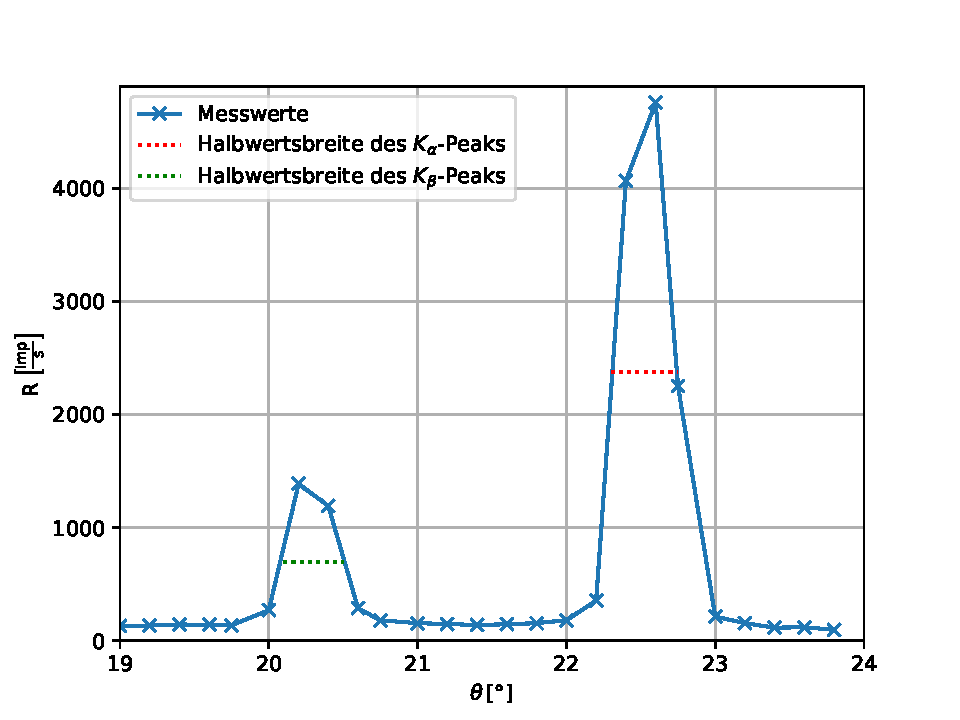
\includegraphics{content/Plots/Detailspektrum.pdf}
  \caption{Detailspektrum der Cu-Röhre der $K_{\alpha}-$ und $K_{\beta}$-Linien.}
  \label{fig:Detailspektrum}
\end{figure}
Durch die jeweils zwei Schnittpunkten mit der Halbwertsbreite und der $K_{\alpha}$- und $K_{\beta}$-Linien 
ergeben sich zu jedem Peak zwei Winkel. Für die $K_{\alpha}$-Linie ergeben sich $\theta_{\alpha,\text{min}}= 22,30\,\unit{\degree}$
und $\theta_{\alpha,\text{max}}= 22,75\,\unit{\degree}$. Für die $K_{\beta}$-Linie sind die Winkel  $\theta_{\alpha,\text{min}}= 20,10\,\unit{\degree}$
und $\theta_{\alpha,\text{max}}= 20,50\,\unit{\degree}$. Aus diesen Winkeln werden mit den Gleichungen (\ref{eqn:lambda}) und (\ref{eqn:E_kin}) die Energien ermittelt. 
Die daraus ergebenen Energiedifferenzen $\Delta E$ wird für die Berechnung des Auflösungsvermögens mit
$$A=\frac{E}{\Delta E}$$
verwendet. Hier beschreibt $E$ die Energie der Peaks. In der Tabelle (\ref{tab:Auflösungsvermögen}) sind die berechneten
Werte aufgelistet.
\begin{table}[H]
  \centering
  \caption{Werte zur Bestimmung der Auflösungsvermögen.}
  \label{tab:Auflösungsvermögen}
  \begin{tblr}{colspec={c c c c}}
      \toprule
      $K$-Linie& $E\,[\unit{\kilo\eV}]$ & $\Delta E\,[\unit{\kilo\eV}]$ & $A$\\
      \midrule
      $\alpha$ &   $8,00$&     $0,15$ &   $52,63$\\
      $\beta$ &    $8,91$&     $0,17$ &   $53,23$\\
      \bottomrule
  \end{tblr}
\end{table}
Mit den Werten aus Tabelle (\ref{tab:Auflösungsvermögen}) und den Gleichungen (\ref{eqn:Kupfer_Linien_Energien_abs}), (\ref{eqn:Kupfer_Linien_Energien_alpha})
und (\ref{eqn:Kupfer_Linien_Energien_beta}) werden die Abschirmkonstanten 
ermittelt. Diese sind in der Tabelle (\ref{tab:Abschirmkonstante}) aufgeführt.
Zudem lässt sich die Absorptionsenergie nicht experimentell bestimmen,
weswegen der Theoriewert $E_{K,\text{abs}}= 8,987\unit{\kilo\eV}$ \cite{Recherche} verwendet wird.
\begin{table}[H]
  \centering
  \caption{Experimentelle und theoretische Abschirmkonstanten.}
  \label{tab:Abschirmkonstante}
  \begin{tblr}{colspec={c c c }}
      \toprule
      $\sigma_{\text{n}}$ & experimentell & theoretisch\\
      \midrule
      $\sigma_1$ &   &     $3,57$ \\
      $\sigma_2$ &    $12,22$&     $12,14$ \\
      $\sigma_3$ &    $22,09$&     $24,04$ \\
      \bottomrule
  \end{tblr}
\end{table}
\subsection{Absorptionsspektrum fünf verschiedener Materialien}
Die Messdaten bei der Messung der Absorptionsspektren sind in den Abbildungen (\ref{fig:Zink}),
(\ref{fig:Gallium}), (\ref{fig:Brom}),(\ref{fig:Strontium}), (\ref{fig:Zirkonium}) dargestellt.
Zusätzlich sind in den Abbildungen die Mittelwerte, sowie der Braggwinke $\theta_K $ markiert. 
Mithilfe der Gleichung (\ref{eqn:Bragg_Bedingung}), (\ref{eqn:lambda}), (\ref{eqn:E_kin}) und (\ref{eqn:sigma_k}) werden die Braggwinkel, die Absorptionsenergien und die Abschirmkonstanten der 
verschiedenen Absorber bestimmt und in der Tabelle (\ref{tab:Abschirmkonstante}) aufgeführt. 
\begin{table}[H]
  \centering
  \caption{Bragg-Winkel, Absorptionsenergie und Abschirmkonstanten der unterschiedlichen Absorber.}
  \label{tab:Abschirmkonstante}
  \begin{tblr}{colspec={c c c c c c c }}
      \toprule
      Material & $\theta_K^{\text{exp.}}\,[\unit{\degree}]$ & $\theta_K^{\text{lit.}}\,[\unit{\degree}]$ & $E_K^{\text{exp.}}\,[\unit{\kilo\eV}]$ & $E_K^{\text{lit.}}\,[\unit{\kilo\eV}]$ & $\sigma_K^{\text{exp.}}$ & $\sigma_K^{\text{lit.}}$\\
      \midrule
      Zn &    $19,84$&  $18,60$  &  $9,07$  & $9,65$   & $4,67$ & $3,56$\\
      Ga &    $17,21$&  $16,06$  &  $10,40$ & $11,11$  & $3,87$ & $3,67$\\
      Br &    $13,13$&  $13,20$  &  $13,55$ & $13,48$  & $4.10$ & $3,83$\\
      Sr &    $10,99$&  $11,01$  &  $16,15$ &  $16,12$ & $4,33$ & $3,98$\\
      Zr &    $9,91$ &  $9,84$   &  $17,89$ &  $18,01$ & $4,61$ & $4,08$\\
      \bottomrule
  \end{tblr}
\end{table}
\begin{figure}[H]
  \centering
  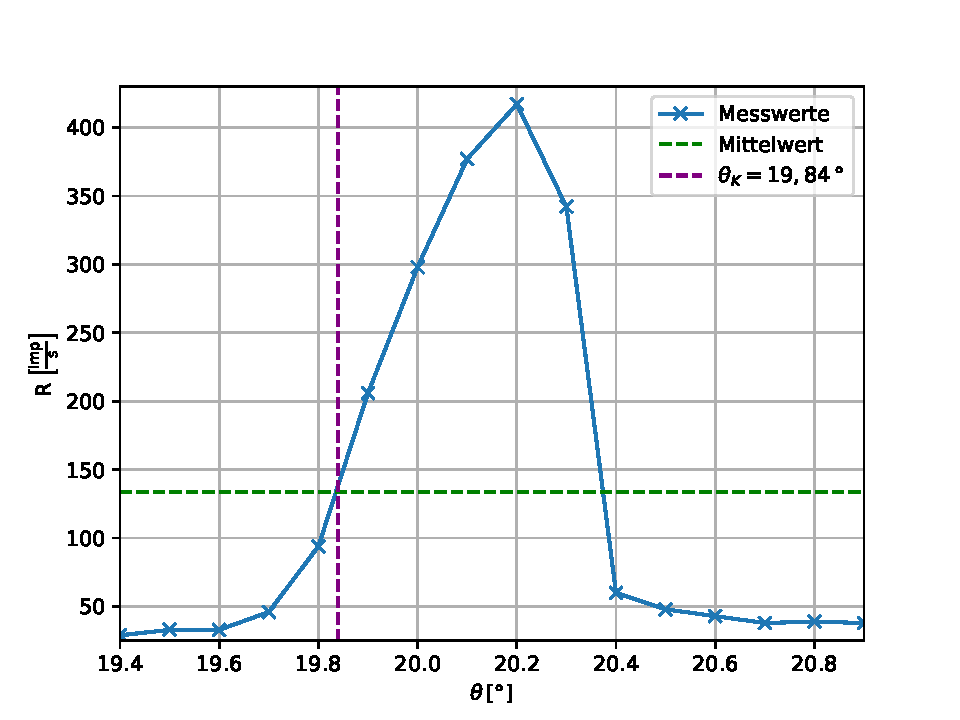
\includegraphics[width=0.80\textwidth]{content/Plots/Zink.pdf}
  \caption{Ermittlung des Braggwinkels des Zink-Absorbers.}
  \label{fig:Zink}
\end{figure}
\begin{figure}[H]
  \centering
  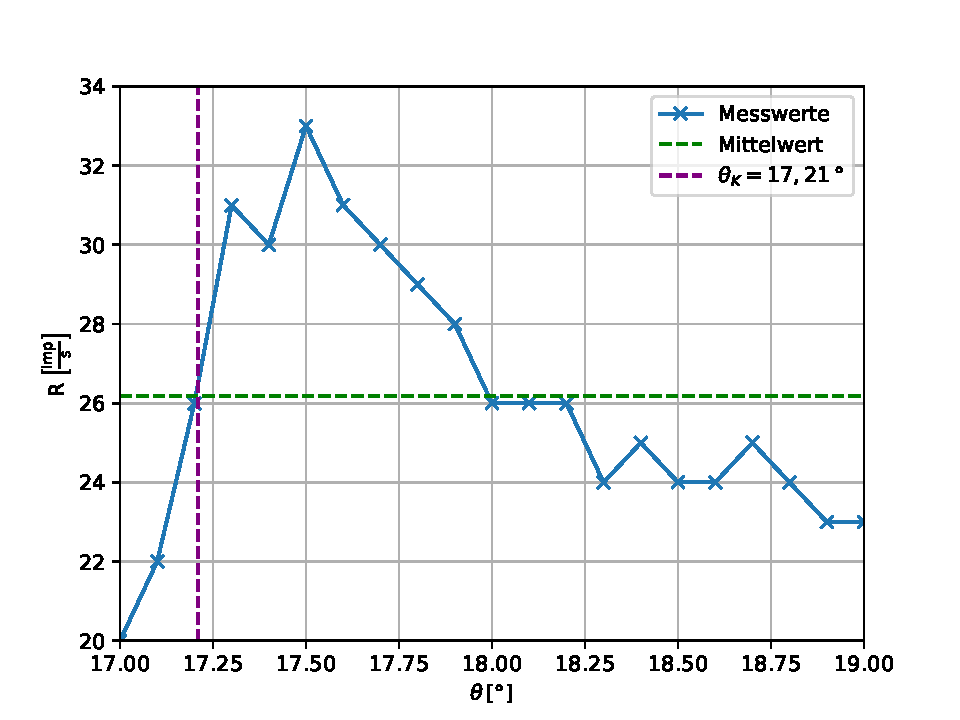
\includegraphics[width=0.80\textwidth]{content/Plots/Gallium.pdf}
  \caption{Ermittlung des Braggwinkels des Gallium-Absorbers.}
  \label{fig:Gallium}
\end{figure}
\begin{figure}[H]
  \centering
  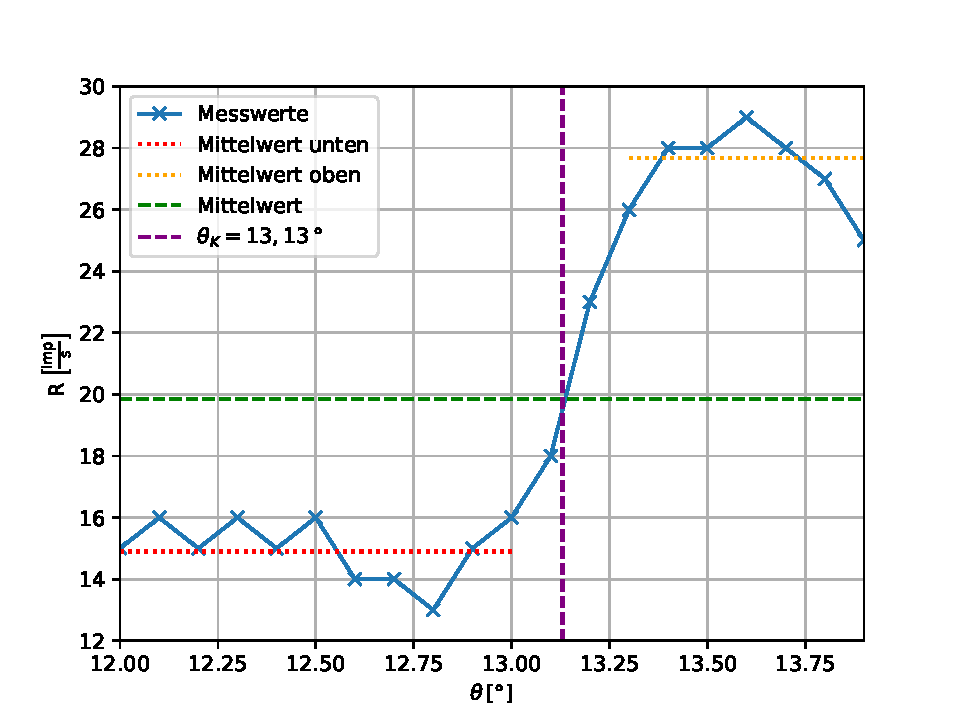
\includegraphics[width=0.80\textwidth]{content/Plots/Brom.pdf}
  \caption{Ermittlung des Braggwinkels des Brom-Absorbers.}
  \label{fig:Brom}
\end{figure}
\begin{figure}[H]
  \centering
  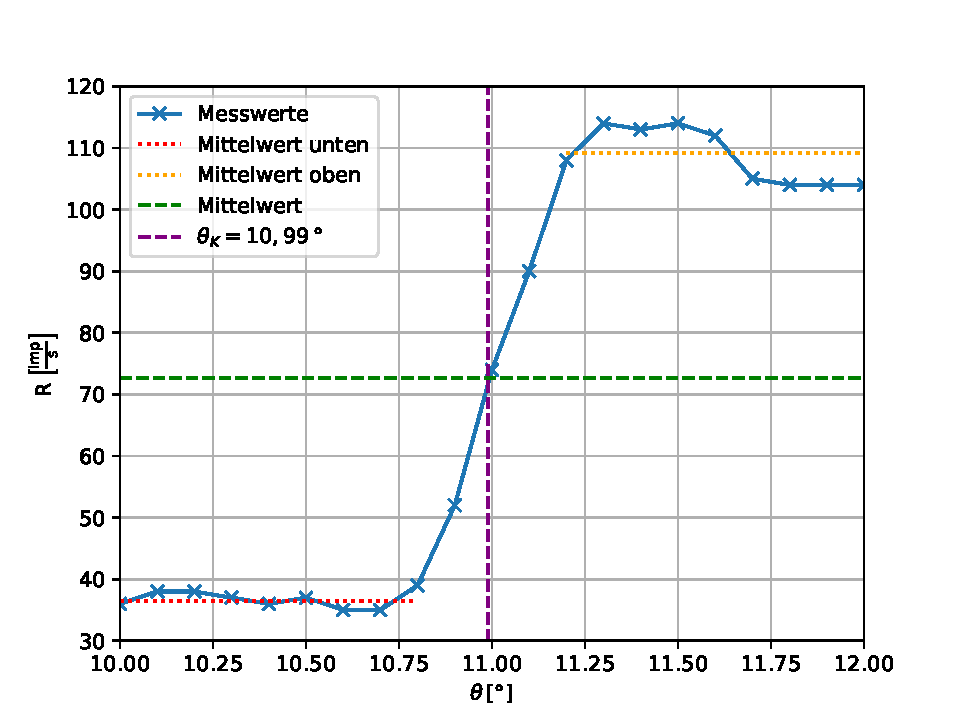
\includegraphics[width=0.80\textwidth]{content/Plots/Strontium.pdf}
  \caption{Ermittlung des Braggwinkels des Strontium-Absorbers.}
  \label{fig:Strontium}
\end{figure}
\begin{figure}[H]
  \centering
  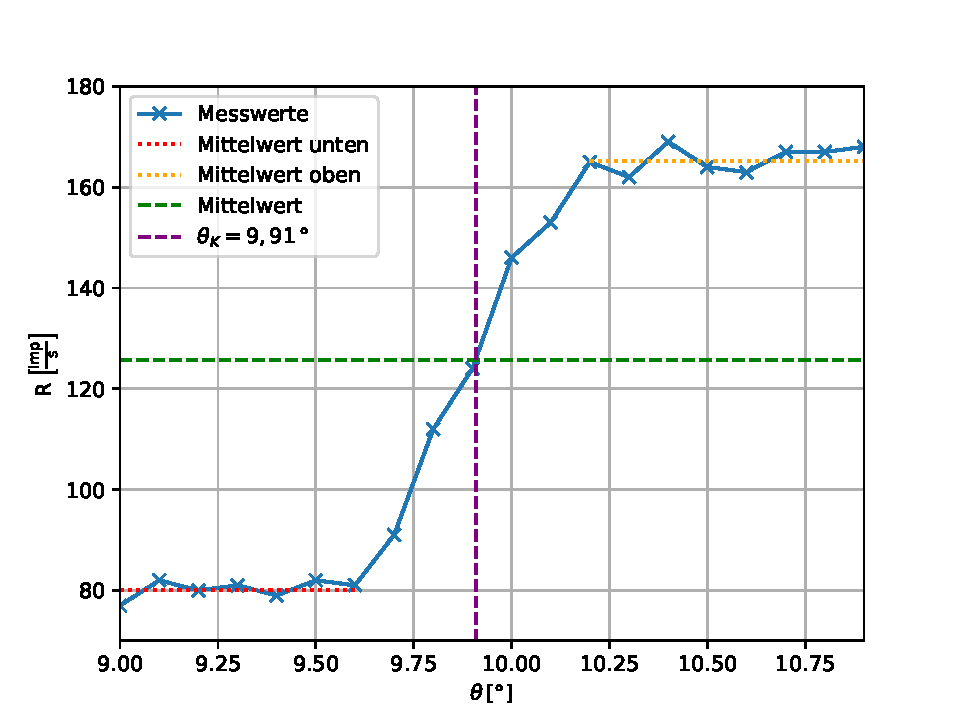
\includegraphics[width=0.80\textwidth]{content/Plots/Zirkonium.pdf}
  \caption{Ermittlung des Braggwinkels des Zirconium-Absorbers.}
  \label{fig:Zirkonium}
\end{figure}
\subsection{Bestimmung der Rydbergkonstanten}
Anhand des Moseleyschen Gesetz (\ref{Bindungsenergie_Elektronen}) lässt sich ein linearer Zusammenhang zwischen
$\sqrt{E_K}$ und $z_{\text{eff}}$ ablesen, wobei der Proportionalitätsfaktor die Rydbergenergie
$R_{\infty}$ entspricht. Daher werden mithilfe der Messdaten der Absorptionsspektren einer 
lineare Regression durchgeführt. Hierfür wird die Funktion
$y =mx+b$ verwendet. Somit ergeben sich 
\begin{align*}
  m=(3,828\pm0,009)\,\sqrt{\unit{\eV}}\\
  b=(-1,81\pm0,28)\,\sqrt{\unit{\eV}}\,.\\
\end{align*}
Demnach lautet die experimentelle Rydbergenergie 
$$R_{\infty,\text{exp}} = m^2=(14,65\pm0,07)\,\unit{\eV}\,.$$
\begin{figure}[H]
  \centering
  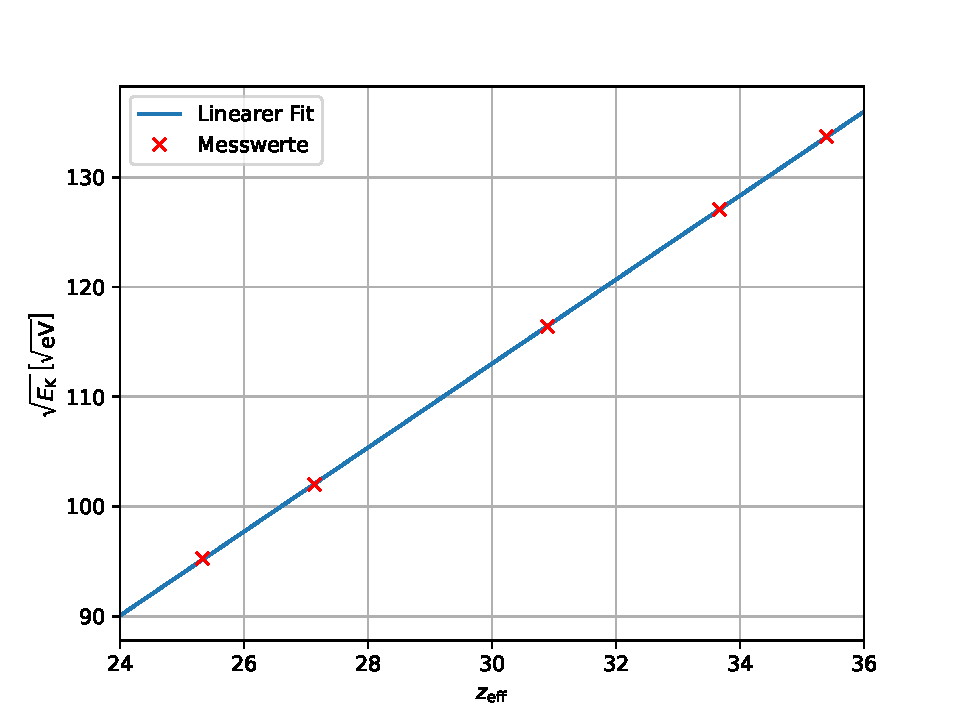
\includegraphics[width=\textwidth]{content/Plots/Rydberg.pdf}
  \caption{Lineare Regression der Absorptionsenergien und die entsprechenden Ordnungszahlen.}
  \label{fig:Rydberg}
\end{figure}
% \begin{figure}
%   \centering
%   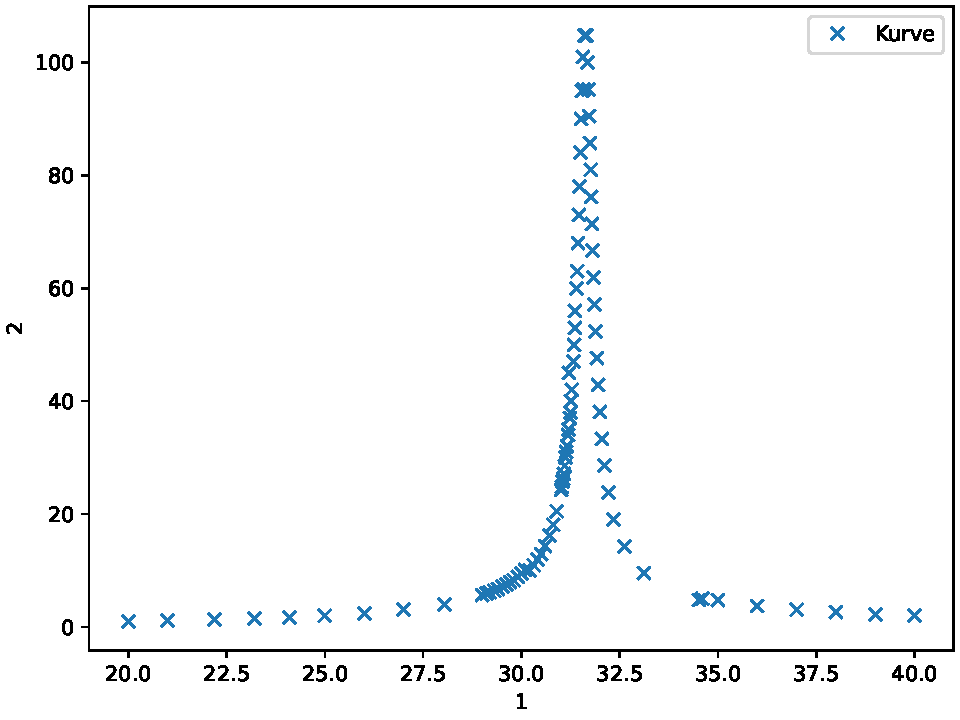
\includegraphics{plot.pdf}
%\label{fig:plot}
% \end{figure}
